%========================PREPARATION===================================
\section{Preparation} \label{appendix:preparation}

\subsection{First preparation} \label{appendix:firstpreparation}
\FloatBarrier
\begin{figure}[ht]
    \begin{center}
    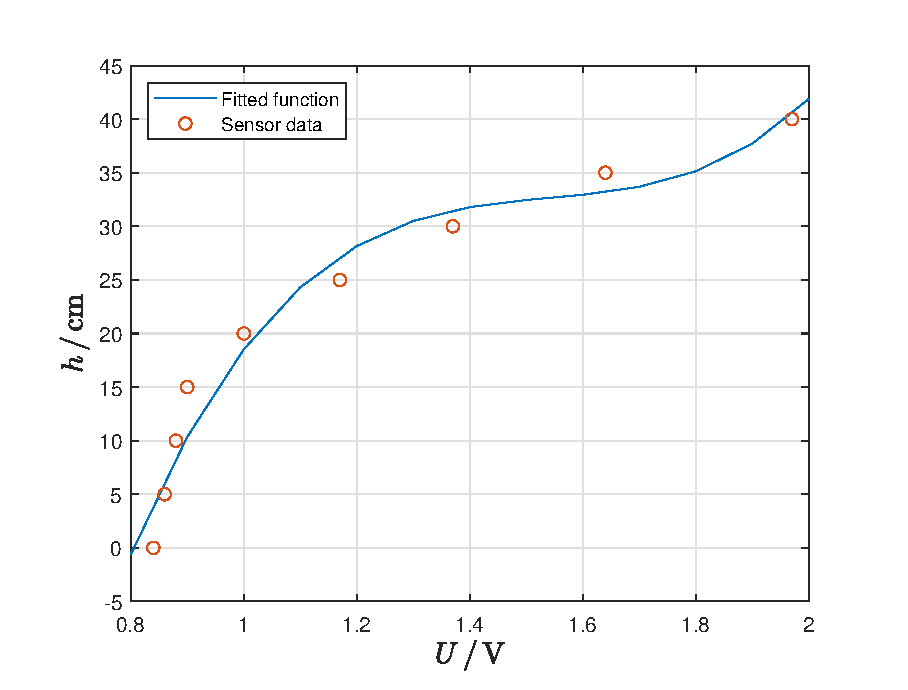
\includegraphics[angle=0,width=0.6\textwidth]{figure/fittedFunction.eps}
    \end{center}
    \caption[Fitted function for first lab preparation]
    {Fitted function $h(u) = (73.36 \cdot u^3) + (-339.13 \cdot u^2) + (527.23 \cdot u) + (-242.94)$}
    \label{fig:fittedFunction}
\end{figure}
\FloatBarrier

\subsection{Second preparation} \label{appendix:secondpreparation}
\FloatBarrier
\begin{figure}[ht]
	\begin{center}
        % trim = left bottom right top
		\includegraphics[clip, trim=0cm 5cm 0cm 5cm, width=1\textwidth]{simulink/simulinkSimulation.pdf}
		\caption[Simulink simulation of the control system]{Simulink simulation of the control system}
		\label{fig:simuSimulation}
	\end{center}
\end{figure}
\FloatBarrier

\FloatBarrier
\begin{figure}[ht]
	\begin{center}
        % trim = left bottom right top
		\includegraphics[clip, trim=0cm 10cm 0cm 8cm, width=1\textwidth]{simulink/simulinkModel.pdf}
		\caption[Simulink model of the system]{Simulink model of the system}
		\label{fig:simuModel}
	\end{center}
\end{figure}
\FloatBarrier

\FloatBarrier
\begin{figure}[ht]
	\begin{center}
        % trim = left bottom right top
		\includegraphics[clip, trim=0cm 8cm 0cm 8cm, width=1\textwidth]{simulink/simulinkController.pdf}
		\caption[Simulink controller]{Simulink controller}
		\label{fig:simuController}
	\end{center}
\end{figure}
\FloatBarrier

\FloatBarrier
\begin{figure}[ht]
	\begin{center}
        % trim = left bottom right top
		\includegraphics[clip, trim=0cm 6.5cm 0cm 6cm, width=1\textwidth]{simulink/simulinkObserver.pdf}
		\caption[Simulink observer]{Simulink observer}
		\label{fig:simuObserver}
	\end{center}
\end{figure}
\FloatBarrier

\FloatBarrier
\begin{figure}[ht]
    \centering
    \begin{subfigure}[b]{0.45\textwidth}
    \includegraphics[width=\textwidth]{simulink/simulinkPlotStepController.eps}
    \caption{}
    \label{subfig:stepController}
    \end{subfigure}
    \begin{subfigure}[b]{0.45\textwidth}
    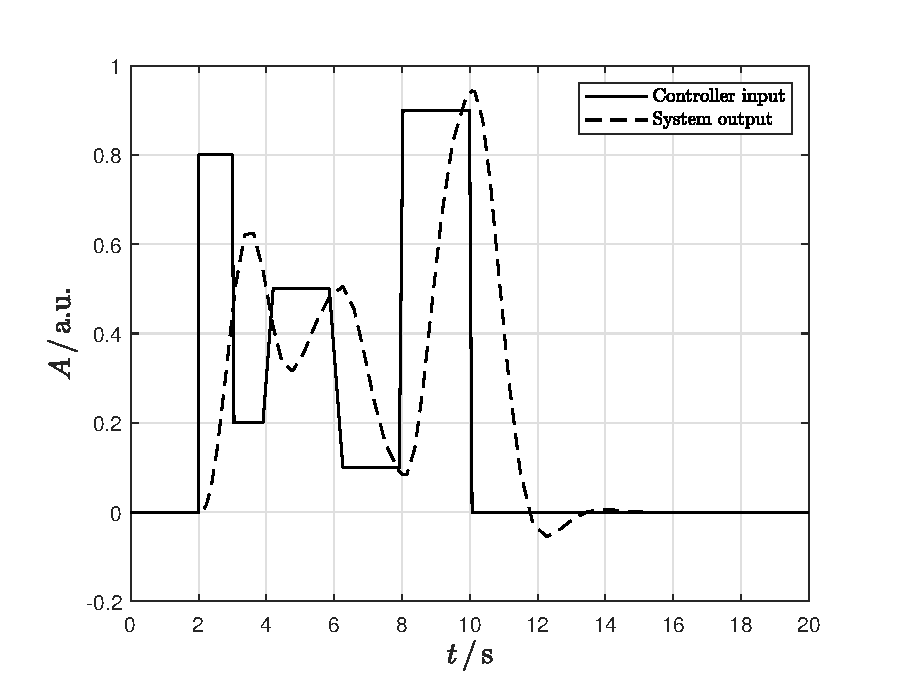
\includegraphics[width=\textwidth]{simulink/simulinkPlotTrajectoryController.eps}
    \caption{}
    \label{subfig:trajController}
    \end{subfigure}

    \hfill
    
    \begin{subfigure}[b]{0.45\textwidth}
    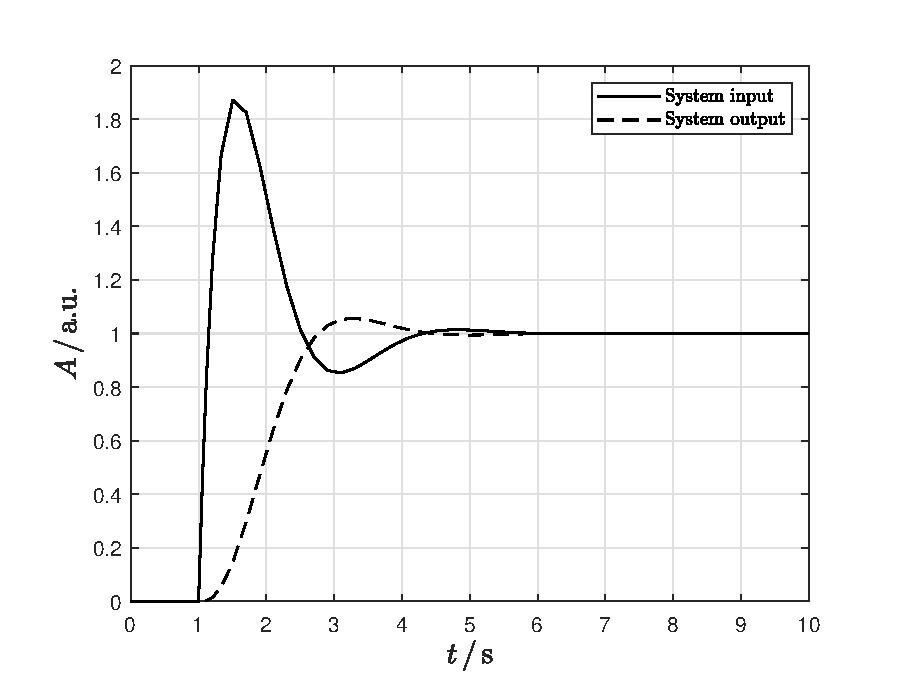
\includegraphics[width=\textwidth]{simulink/simulinkPlotStepSystem.eps}
    \caption{}
    \label{subfig:stepSystem}
    \end{subfigure}
    \begin{subfigure}[b]{0.45\textwidth}
    \includegraphics[width=\textwidth]{simulink/simulinkPlotTrajectorySystem.eps}
    \caption{}
    \label{subfig:trajSystem}
    \end{subfigure}

    \hfill
    
    \begin{subfigure}[b]{0.45\textwidth}
    \includegraphics[width=\textwidth]{simulink/simulinkPlotStepObserver.eps}
    \caption{}
    \label{subfig:stepObserver}
    \end{subfigure}
    \begin{subfigure}[b]{0.45\textwidth}
    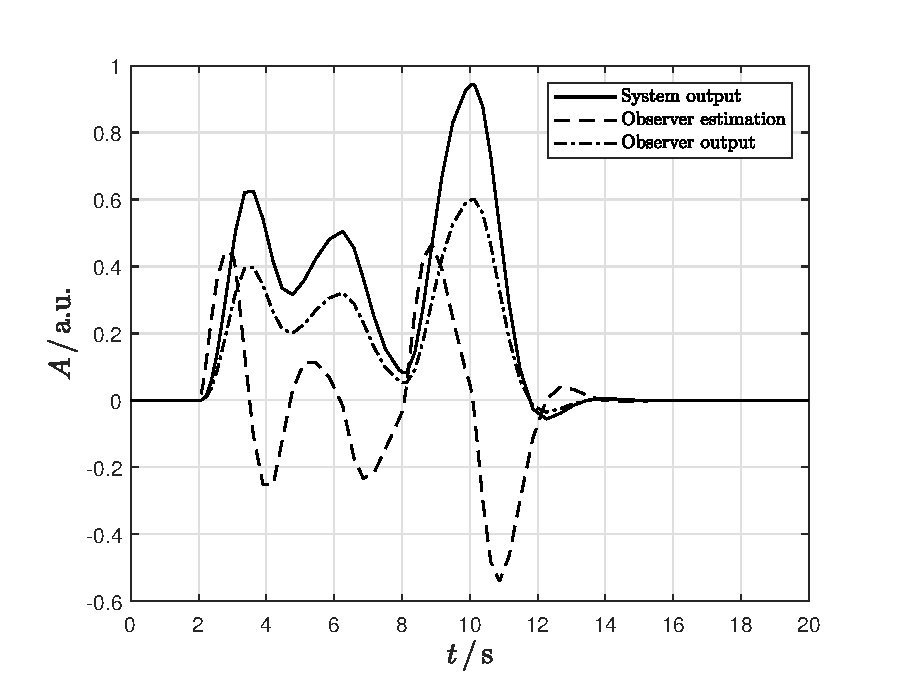
\includegraphics[width=\textwidth]{simulink/simulinkPlotTrajectoryObserver.eps}
    \caption{}
    \label{subfig:trajObserver}
    \end{subfigure}

    \hfill
    
    \caption[Simulations in Simulink]{Left for step input with (a) controller (c) system and (e) observer. Right trajectory input with (b) controller (d) system and (f) observer.}
    \label{fig:simulations}
\end{figure}
\FloatBarrier


\newpage


%========================DATA===================================
\section{Laboratory} \label{appendix:data}

\subsection{Sensor data} \label{appendix:sensordata}
\begin{table}[H]
\caption[Sensor output voltage against distance]{Sensor output voltage against distance} \label{tab:sensor}
\begin{center}
\begin{tabular}{ c c }
\toprule
Distance & Sensor voltage \\
\midrule\\
18  & 1.93 \\
23  & 1.91 \\
28  & 1.68 \\
33  & 1.32 \\
38  & 1.11 \\
43  & 0.96 \\
48  & 0.90 \\
53  & 0.88 \\
58  & 0.82 \\
\bottomrule
\end{tabular} 
\end{center}
\end{table} 

\FloatBarrier
\begin{figure}[ht]
    \begin{center}
    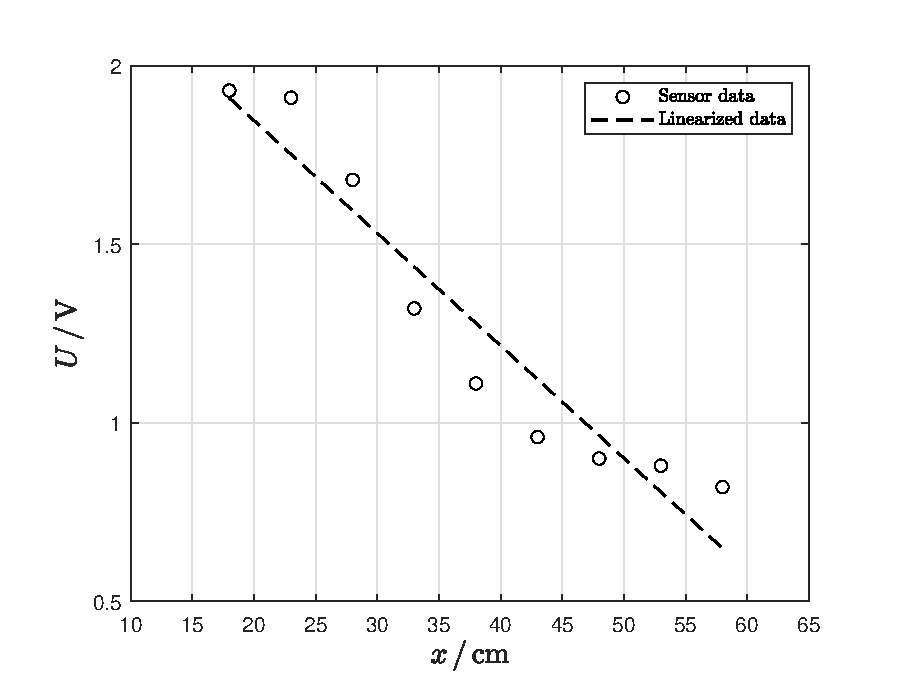
\includegraphics[angle=0,width=0.6\textwidth]{figure/sensorLinearized.eps}
    \end{center}
    \caption[Sensor linearization]
    {Sensor linearization: $f(x) = -0.0315*x + 2.4758888$}
    \label{fig:sensorLinearization}
\end{figure}
\FloatBarrier

\newpage

\subsection{System identification} \label{appendix:systemidentification}
\FloatBarrier
\begin{figure}[ht]
    \centering
    \begin{subfigure}[b]{0.45\textwidth}
    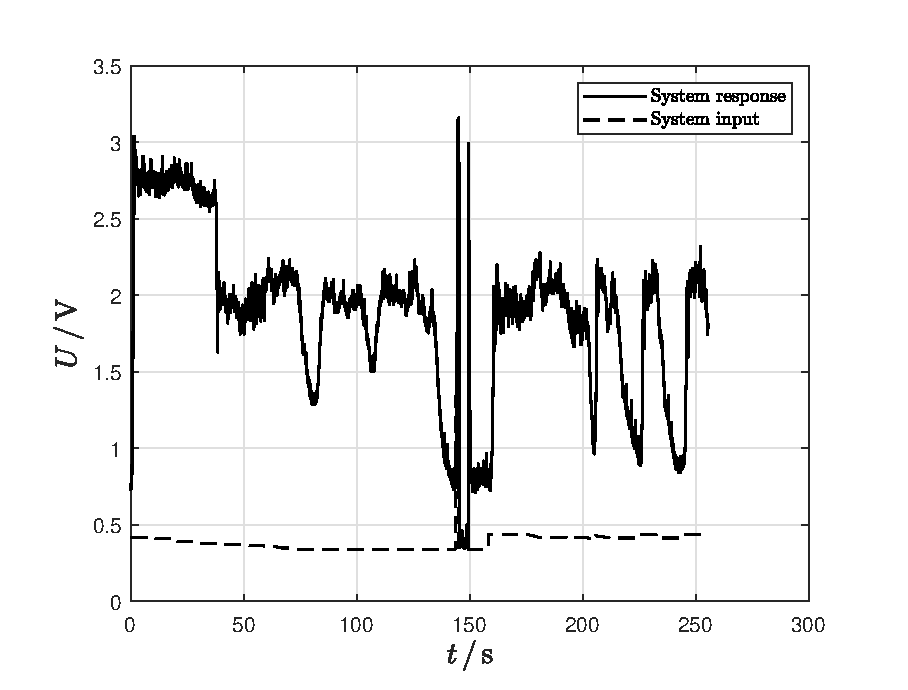
\includegraphics[width=\textwidth]{figure/raw.eps}
    \caption{}
    \label{subfig:raw}
    \end{subfigure}
    \begin{subfigure}[b]{0.45\textwidth}
    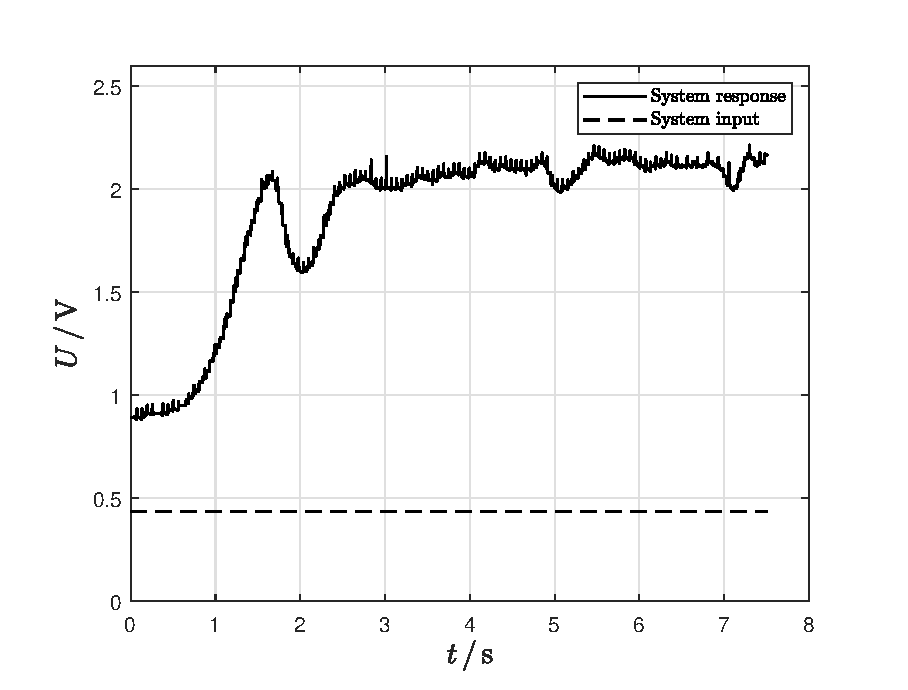
\includegraphics[width=\textwidth]{figure/trimming.eps}
    \caption{}
    \label{subfig:trimming}
    \end{subfigure}

    \hfill
    
    \begin{subfigure}[b]{0.45\textwidth}
    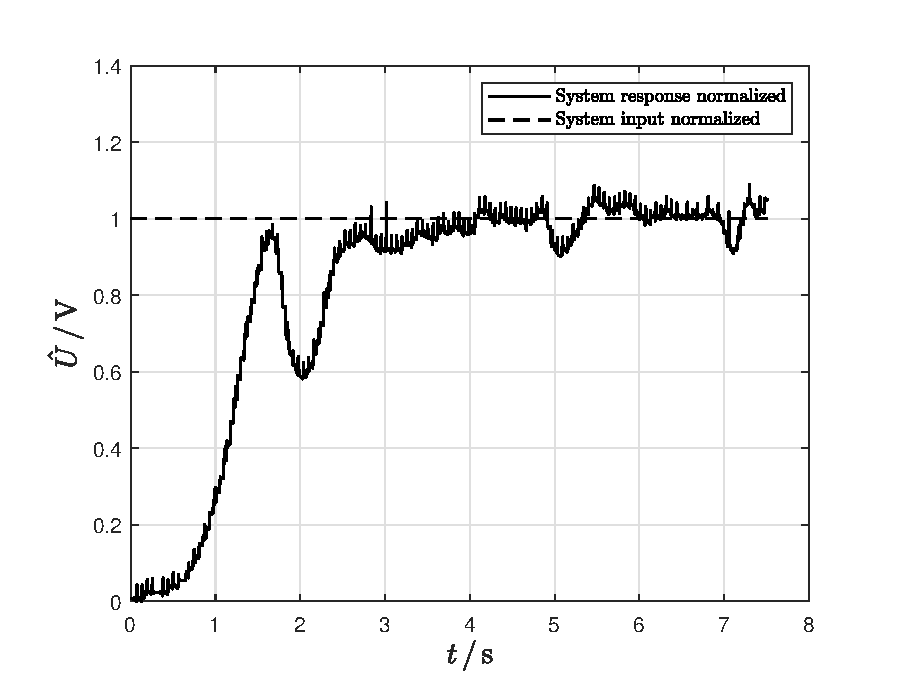
\includegraphics[width=\textwidth]{figure/normalize.eps}
    \caption{}
    \label{subfig:normalize}
    \end{subfigure}
    \begin{subfigure}[b]{0.45\textwidth}
    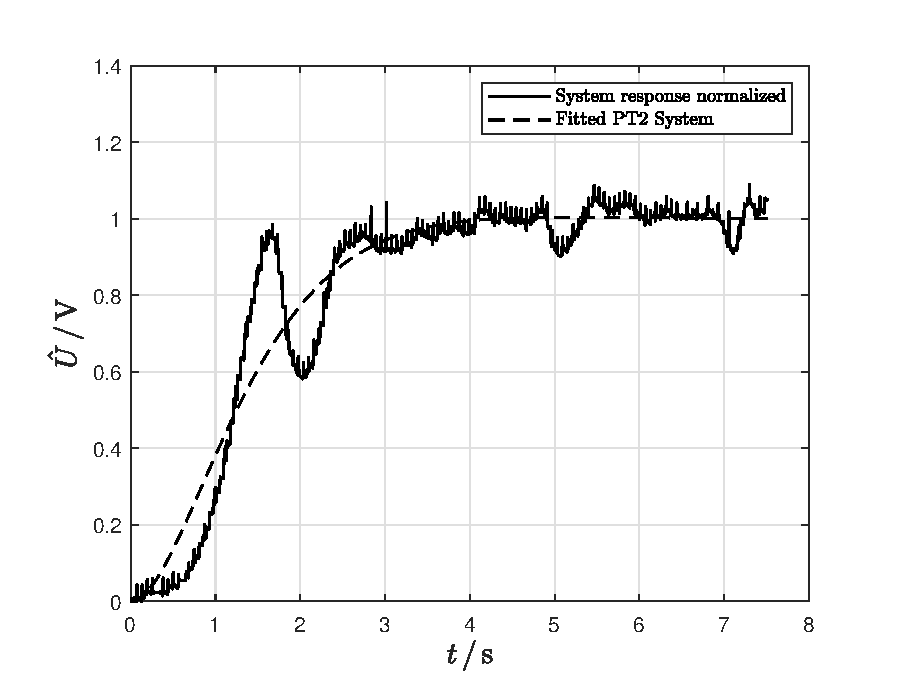
\includegraphics[width=\textwidth]{figure/fitting.eps}
    \caption{}
    \label{subfig:fitting}
    \end{subfigure}

    \hfill
    
    \caption[System identification in the laboratory]{(a) Raw data (b) Trimmed (c) Normalized (d) Fitted PT2 system}
\end{figure}
\FloatBarrier

\newpage

\subsection{Controller performance} \label{appendix:performance}
\FloatBarrier
\begin{figure}[ht]
	\begin{center}
        % trim = left bottom right top
		\includegraphics[clip, trim=0cm 6cm 0cm 6cm, width=0.8\textwidth]{simulink/simulinkLaboratory.pdf}
		\caption[Simulink laboratory application]{Simulink laboratory application}
		\label{fig:simuLaboratory}
	\end{center}
\end{figure}
\FloatBarrier

\FloatBarrier
\begin{figure}[ht]
    \begin{center}
    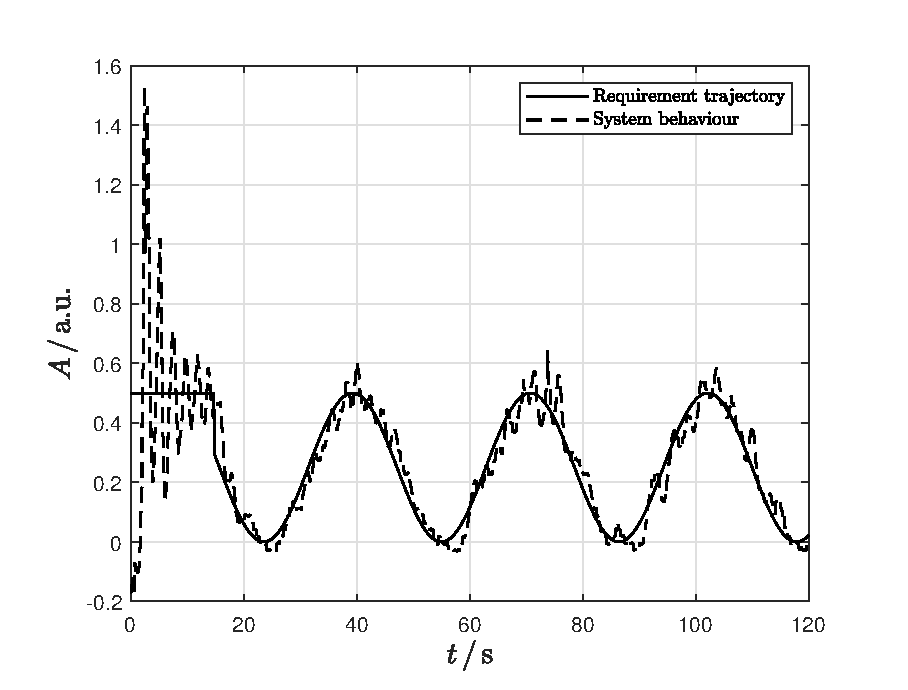
\includegraphics[angle=0,width=0.6\textwidth]{simulink/simulinkPlotTrajectoryLaboratory.eps}
    \end{center}
    \caption[System behaviour with sine wave trajectory]
    {System behaviour with sine wave trajectory}
    \label{fig:simuSineTrajectory}
\end{figure}
\FloatBarrier


\newpage


%========================MATLAB===================================
\section{MATLAB} \label{appendix:matlab}

\subsection{First laboratory}
\lstinputlisting[style=MStyle]{m_files/laboratory.m}
\subsubsection{Plots}
\lstinputlisting[style=MStyle]{m_files/plots.m}
\subsubsection{PT2 fitting function}
\lstinputlisting[style=MStyle]{m_files/unit_step_PT2.m}

\newpage

\subsection{Second laboratory}
\lstinputlisting[style=MStyle]{m_files/laboratory1.m}